\paragraph{In executed quantity and money.} For a \emph{known} pair (one group at rate $\eta$ against two at $\eta\pm\delta$ with the same total weight), the information needed can be stated in trades. The executed quantity a prober needs is of exact order $\delta^{-2}$: the two price responses first differ at lag two, by $-\kappa^2q\delta^2$, and a single pulse of size $2\sigma\Phi^{-1}(1-\alpha)/(\kappa^2q\delta^2)$ attains error $\alpha$. The capital a counterparty must post to fill such probes is of order $\delta^{-4}$, because the adverse mark of a probe grows with the square of its size. Halving the difference between two memories therefore quadruples the trading needed and multiplies the capital by sixteen (Theorems~\ref{thm:quantity} and~\ref{thm:cap} and Lemma~\ref{thm:capital}, Supplement~\ref{app:capital}).

\paragraph{Near instability.} Theorem~\ref{prop:passive} is stated on a family that stays uniformly stable. One might hope that the barrier lifts as the market approaches instability, since the loop then amplifies every difference. It does not. What becomes visible is the distance to instability, not the composition.

\begin{proposition}[The barrier does not lift near instability]\label{prop:nearcrit}
Fix $K\ge2$ and the $K$-group Gauss and Gauss--Radau economies $A$ and $B$ of Theorem~\ref{thm:kcohort}, with positive weights, rates in $(0,1)$ and $\kappa>0$. For a margin $\epsilon>0$, choose persistences $a_A(\epsilon)$ and $a_B(\epsilon)$ so that both economies have feedback budget $S=1-\epsilon$, and suppose $a_A(\epsilon),a_B(\epsilon)>0$ for $\epsilon\le\epsilon_0$. Let $D_\epsilon(B\|A)$ be the Kullback--Leibler divergence rate between the stationary price processes driven by i.i.d.\ $N(0,\sigma^2)$ innovations. There is $C$, not depending on $\epsilon$ or $\Delta\eta$, such that
\[
D_\epsilon(B\|A)\ \le\ C\,(\Delta\eta)^{4K-2}\qquad\text{for all }0<\epsilon\le\epsilon_0\text{ and all small }\Delta\eta .
\]
\end{proposition}

\paragraph{In words.} Even as the market approaches a crash, passive prices reveal no more about who is trading than they did in calm conditions, per observation. They reveal more and more about how close the market is to instability: if the two economies share the persistence $a$ instead of the budget, their budgets differ by order $(\Delta\eta)^{2K-1}$, and numerically the divergence rate then grows like $\epsilon^{-1}$. The proof is in Supplement~\ref{app:nearcrit}. Two limits apply. The statement is about the divergence rate per observation; near instability prices are strongly dependent, and a finite-sample bound that is uniform in $\epsilon$ is not proved, although numerically the exact information in $n$ observations stays within $3\%$ below $n$ times the rate down to $\epsilon=10^{-3}$ (Supplement~\ref{app:nearcrit}). And probing does gain near instability: the squared response difference grows like $\epsilon^{-1}$ (numerical, \nolinkurl{research_extension/fragility_reveals}), but probing a market at the edge of instability is not a policy. Figure~\ref{fig:barrier} shows both statements.

\begin{figure}[t]
\centering
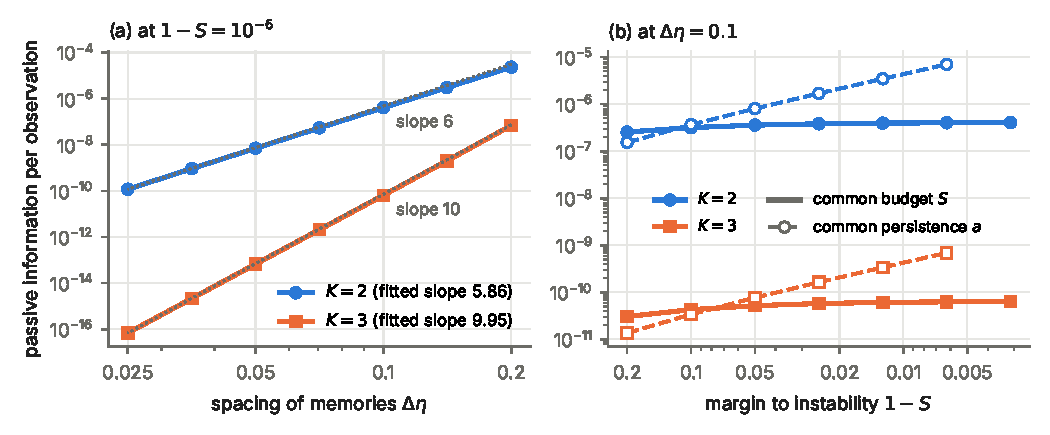
\includegraphics[width=\textwidth]{fig_barrier.pdf}
\caption{The passive barrier near instability. Both panels show the Gaussian Kullback--Leibler information per observation between the stationary price processes of two populations whose merged measures are the $K$-node Gauss and Gauss--Radau rules on memories spread over $\Delta\eta$ around $0.5$ (total weight $0.3$, impact $\kappa=0.5$). (a)~At a common feedback budget one millionth below instability, the information falls like $(\Delta\eta)^{4K-2}$ (dotted lines). (b)~Held at a common budget (solid), the information stays bounded as the margin $1-S$ shrinks; held at a common persistence (dashed), it grows without bound, because the budgets then differ. Computed from the closed-form spectra; scripts in \nolinkurl{research_extension/fragility_reveals/}.}
\label{fig:barrier}
\end{figure}

\paragraph{Monetary value of algorithm tags.} The sample complexity gap converts directly into a dollar value of mandatory class-tagged disclosure. Let $c > 0$ be the per-period opportunity cost of market surveillance or active supervisory probing (e.g., $c = \sigma_w^2 / \bar{\kappa}$ in dollar terms). To attain target statistical power $1-\alpha$, a supervisor without tags must incur passive surveillance expenditure $C_{\mathrm{pass}} = c N_p$, whereas under mandatory class disclosure the expenditure is $C_{\mathrm{tag}} = c N_t$. The monetary Value of Disclosure (VOD) is the avoided surveillance cost:
\begin{equation}\label{eq:vod}
\mathrm{VOD}(K, \Delta\eta, c, N_t) = C_{\mathrm{pass}} - C_{\mathrm{tag}} = c \cdot N_t \left[(\Delta\eta)^{-(4K-2)} - 1\right].
\end{equation}
By Theorem~\ref{thm:discvalue}, this avoided expenditure is non-negative, scales linearly in surveillance cost $c$ and sample size $N_t$, and grows without bound as $\Delta\eta \to 0$ (\texttt{p1\_disclosure\_monetary\_value}, \texttt{p1\_disclosure\_vod\_as\_cost\_difference}, \texttt{p1\_disclosure\_value\_dominates\_audit\_cost}). In financial markets with $K=2$ cohorts and cohort separation $\Delta\eta = 0.1$, the sample complexity ratio is $(\Delta\eta)^{-6} = 10^6$ (\texttt{p1\_disclosure\_ratio\_K2\_delta\_eta01}). At a modest surveillance cost of $c = \$10$ per market-day with $N_t = 100$ tagged records required, passive surveillance would demand $\$10 \times 10^8 = \$1{,}000{,}000{,}000$ in observation expenditure, yielding $\mathrm{VOD} \approx \$10^9$ in averted surveillance waste (\texttt{p1\_disclosure\_vod\_example}, \texttt{p1\_disclosure\_cost\_ratio\_K2}). Any fixed compliance or auditing cost incurred to implement algorithm tagging is therefore dominated by several orders of magnitude.
